\chapter{背景综述}

高性能计算(High Performance Computing)一直是计算机科研领域的重要主题。伴随近20年来超级计算集群
性能和数量的指数式增长,我们的超算能力已经迈进Petaflop时代($10^{15}$次浮点运算), 更强大的
exaflop时代($10^{18}$次浮点运算)也即将到来。但是目前能够有效充分利用超算集群的应用程序还为数
不多,因此超算应用是制约HPC界发展的一大瓶颈。\par
在超算的应用领域,科研活动占据了一大部分,如天文学,粒子物理,计算化学等基础学科;另外在工程和
商业领域也有重要的应用,如汽车,飞机设计中得计算流体力学模拟仿真,油田勘探中的海量信息处理和开采
方案设计以及在商业投资领域的高频交易等。此外随着云计算和大数据相关研究和商业应用的快速崛起,
怎样将高性能计算和数据挖掘分析等技术结合起来也成为了当前超算领域的研究热点。本文的主题是探讨
高性能计算在金融领域的一个重要应用以及其在Intel最新的MIC架构上的实现。首先在中我们将简单介绍
高性能计算和金融领域超算应用的一些基本情况。

\section{高性能计算的诞生和发展} % (fold)
\label{sec:intro-hpc}

高性能计算的概念和实现依赖于算法理论和硬件制造的发展。在算法理论方面,并行运算(Parallel computing)
的研究在70年代就开始,但是受制于当时硬件领域的发展瓶颈,并行运算方面的很多理论没有得到充分地发展。
如图\ref{fig:intelProcessor} 所示,Intel的处理器的在2000年之前晶体管的数量和时钟频率都能依照摩尔定律增长。
\begin{figure}
	\centering
	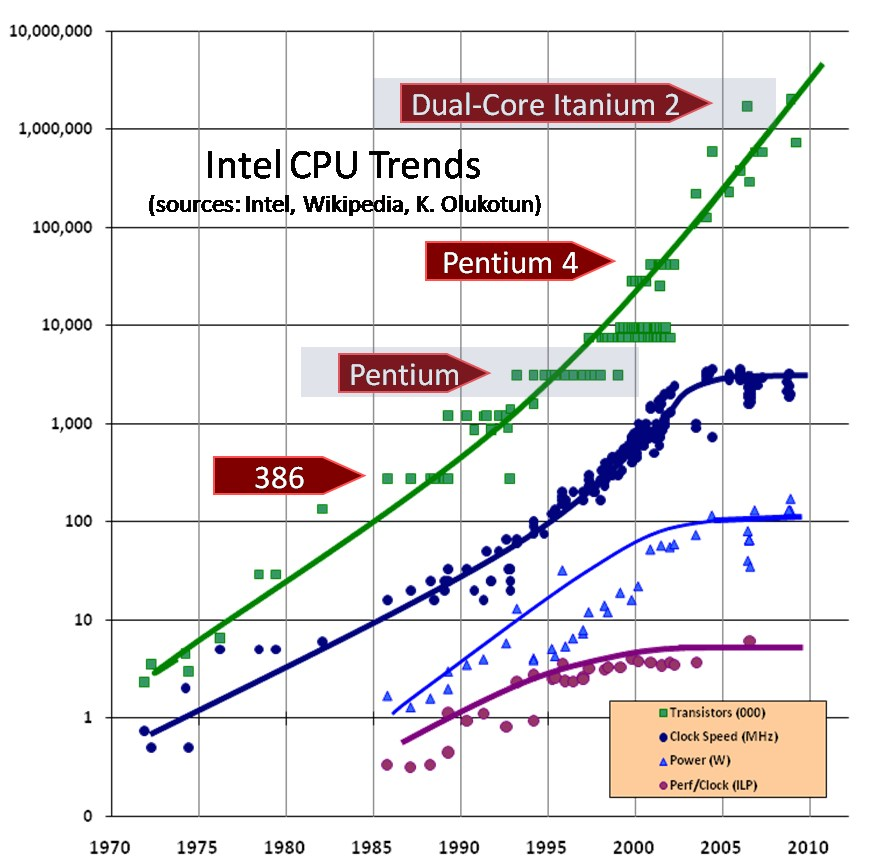
\includegraphics[width=\textwidth]{chap1/Figures/CPU-Scaling.jpg}
	\caption{Intel处理器的发展趋势}
	\label{fig:intelProcessor}
\end{figure}
但是当单个处理器的制造工艺到达纳米级别后,受制于量子效应已经无法进一步提高单个处理器的时钟频率。
随后业界开始转而使用多核系统(Multi-core system),直至目前出现的众核系统(Manycore system)来提升超算的性能。目前最权威的HPC超算
集群排行榜Top500给出的结果显示,无论是排名第一的机器还是所有500强计算能力的综合都较好地符合摩尔定律逐年增长。
\begin{figure}
	\centering
	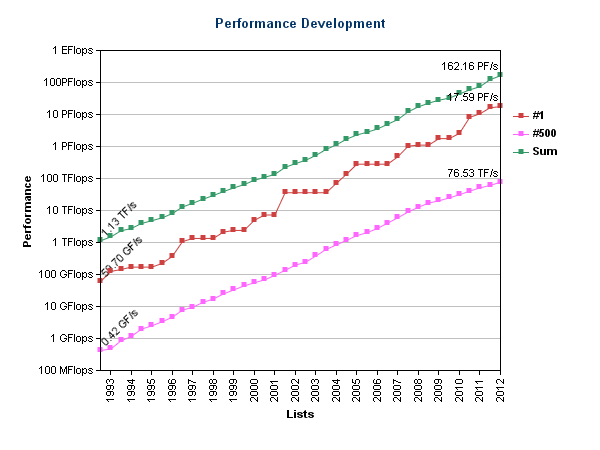
\includegraphics[width=\textwidth]{chap1/Figures/top500Perf.png}
	\caption{Top500超算集群的性能发展}
	\label{fig:top500Perf}
\end{figure}
但是这些峰值运算速度仅仅代表了理论上一台超算集群能够达到的速度,其测试结果也是通过相对简单地基准程序(benchmark)获得的,而真正复杂的应用程序大多数
还未能在超算集群上跑出好的使用效率。制约在超算上展开大规模应用的因素有以下几点。
\begin{enumerate}
    \item 缺少能极大地提供并行性的算法
	\item 数据间的通信受制于内存读取速度和处理器间的连接速度。
	\item 从串行编程模型转到并行编程的学习成本
\end{enumerate}
算法的并行性是最为重要的一点,目前的大多数数学模型和对应的算法没有足够的并行性能够充分发挥超算集群的潜力。我们需要的是面向并行建立新的数学模型和
算法来解决实际问题。同时我们的编程模型和编程语言也需要相应地升级,使之能更自然和原生地支持并行架构。这一点也被认为是同向Exascale计算的关键。
而对于第二点,目前出现的CPU/coprocessor架构已经迈出了重要的一步。Nvidia公司的GPU和GPGPU编程模型可以充分利用GPU的充足带宽(bandwidth)优化数据并行性德问题
(Data Parallel, SIMD),而Intel公司则相应地推出了自己的协处理器Xeon Phi (Many Integrated Core Architecture, MIC Architecture)。Xeon Phi同样拥有强大的
带宽(382G/s)。此外Xeon Phi在编程难度上相比于GPGPU更有利于初学者掌握,实际上用户可以相对简单地从CPU的串行程序过渡到Xeon Phi的并行代码上。
本课题的应用即在MIC架构上展开,并在数据通信等方面进行优化。

% section 高兴能计算的产生和发展 (end)

\section{金融领域的超算应用} % (fold)
\label{sec:intro-finance}


% section 金融领域的超算应用 (end)


